\subsection{Task Assignment}\label{subsubsec:task-assignment}
Given the set of posets~$\mathcal{P}_{\varphi}$ derived from the previous
section, this section describes how this set can be used to compute
the optimal assignment of these subtasks. More specifically, we consider
the following sub-problems of task assignment:

\begin{problem}\label{problem:}
Given any poset $P=(\Omega,\, \preceq_{\varphi},\, \neq_{\varphi})$
where~$P\in \mathcal{P}_{\varphi}$,
find the optimal assignment of all subtasks in~$\Omega$ to the multi-agent system
$\mathcal{N}$ such that
(i) all partial ordering requirements in $\preceq_{\varphi},\, \neq_{\varphi}$ are
respected; (ii) the maximum completion time of all subtasks is minimized.
\hfill $\blacksquare$
\end{problem}



To begin with, even without the requirements of partial ordering
and collaborative actions, the above problem includes the multi-vehicle routing
problem~\cite{gini2017multi, khamis2015multi},
and the job-shop scheduling problem~\cite{brucker1994branch} as special instances.
Both problems are well-known to be NP-hard.
Thus, the above problem is also NP-hard and its most common and straightforward solution
is to formulate a Mixed Integer Linear Program (MILP). 
{However, there are two major drawbacks of MILP:
(i) the computation complexity grows exponentially with the problem size;
(ii) there is often no intermediate solution before the optimal solution is generated via a MILP solver,
, e.g., CPLEX~\cite{lima2010ibm}.
Both drawbacks hinder the usage of this approach in large-scale real-time applications,
where a timely good solution is far more valuable than the optimal solution.}

%========================================
\begin{figure}[t!]
	\centering
	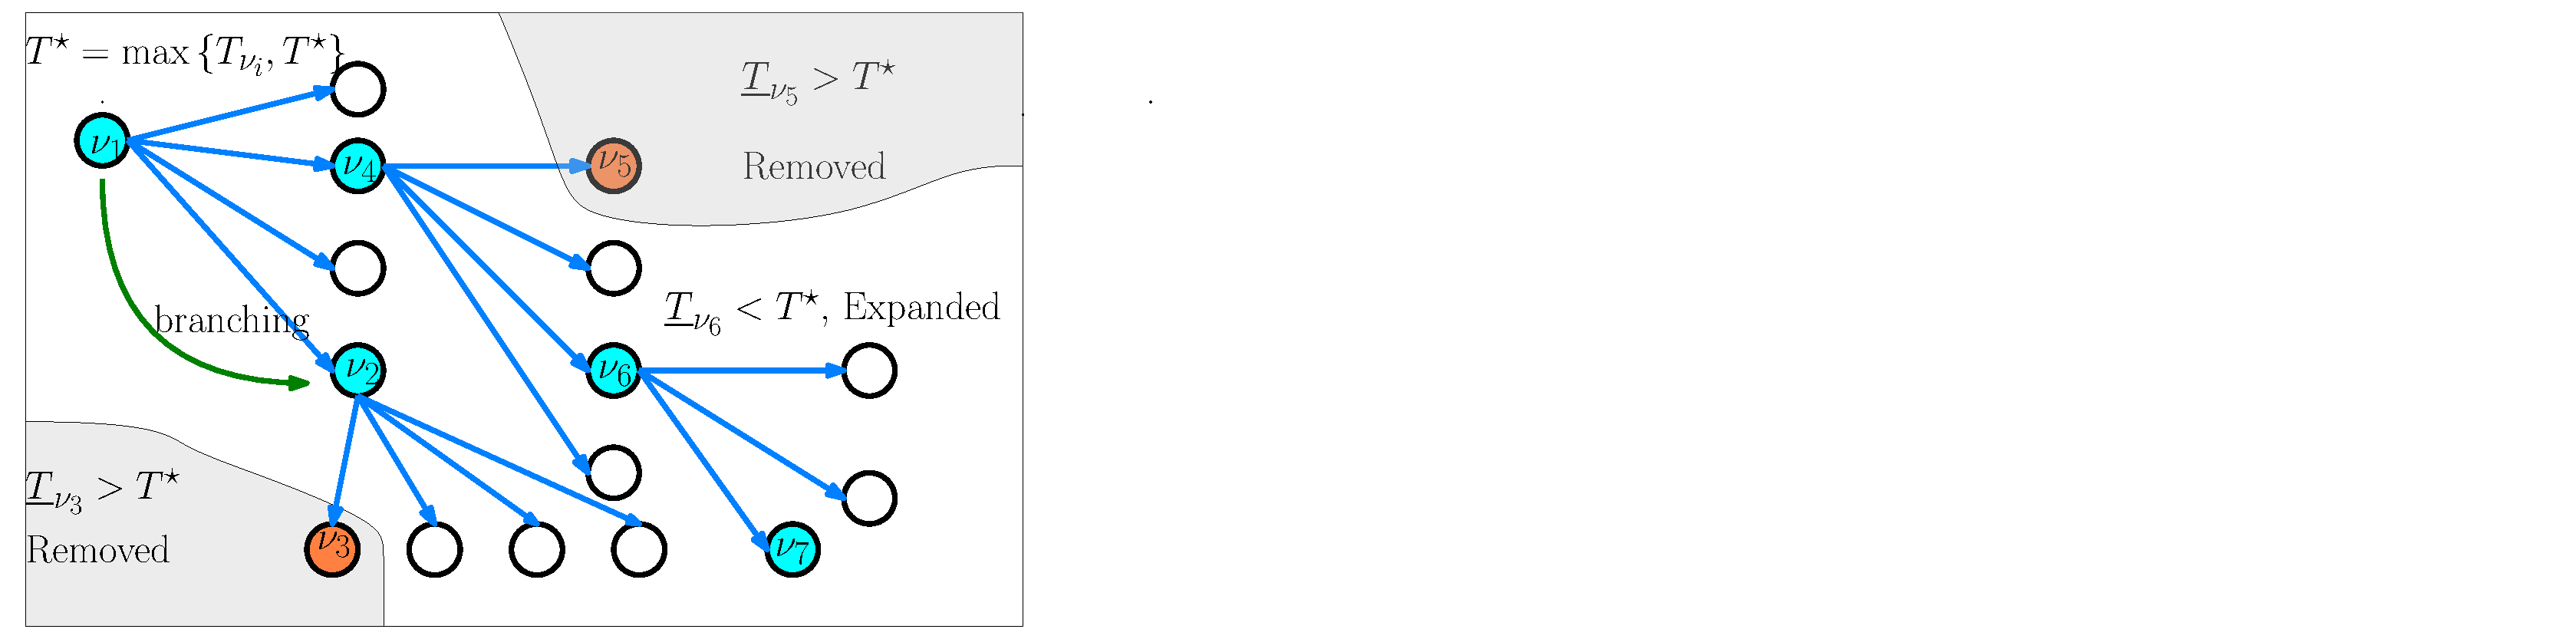
\includegraphics[width=0.9\linewidth]{figures/bnb_graph3.pdf}
	%--------------------
	\caption{
		Illustration of the main components in the BnB search,
		i.e., the node expansion and branching to generate explore new nodes (in green arrow);
		and the lower and upper bounding to avoid undesired branches (in orange).}
	\label{fig:bnb_search_logic}
	%--------------------
\end{figure}
%========================================

Motivated by these observations, an anytime assignment
algorithm is proposed in this work based on the Branch and Bound (BnB) search
method~\cite{lawler1966branch, morrison2016branch}.
It is not only complete and optimal, but also anytime, meaning that a good
solution can be inquired within any given time budget.
As shown in Fig.~\ref{fig:bnb_search_logic},
the four typical components of a BnB
algorithm are the node expansion, the branching method,
and the design of the upper and lower bounds.
These components for our application are described in detail below.


\textbf{Node expansion}.
Each node in the search tree stands for one partial assignment of the
subtasks, i.e.,
\begin{equation}\label{eq:node}
\nu = (\tau_1,\,\tau_2,\cdots,\tau_N),
\end{equation}
where $\tau_n$ is the ordered sequence of tasks assigned to agent~$n\in \mathcal{N}$.
To give an example, for a system of three agents,
$\nu=((\omega_1,\omega_2),(),())$ means that two subtasks
$\omega_1,\, \omega_2$ are assigned to agent~$1$,
whereas no tasks to agents~$2$ and $3$.


To avoid producing infeasible nodes, we assign only the next task satisfies
the partial order. Let~$\nu$ be the current node of the search tree.
The \emph{next} subtask~$\omega$ to be assigned is chosen from the
poset~$\mathcal{G}_{P_\varphi}$ defined in Def.~\ref{def:poset-graph}
if \emph{all} of its parent subtasks are already assigned, i.e.,
\begin{equation}\label{eq:next-task}
\omega' \in \Omega_\nu, \; \forall \omega' \in \text{Pre}(\omega),
\end{equation}
where~$\text{Pre}(\omega)$ is the set of preceding or parenting subtasks of $\omega$ in~$\mathcal{G}_{P_\varphi}$;
and $\Omega_\nu$ is the set of assigned subtasks as
\begin{equation}\label{eq:node-tasks}
\Omega_{\nu}=\{\omega\in\tau_n,\,\forall n\in \mathcal{N}\},
\;\Omega^-_{\nu} = \Omega\backslash \Omega_{\nu},
\end{equation}
where~$\Omega$ is the set of subtasks from $P_\varphi$;
$\Omega_{\nu}$ is the set of subtasks already assigned in node~$\nu$;
and $\Omega^-_{\nu}$ are the remaining unassigned subtasks.Once this 
subtask~$\omega$ is chosen, the succeeding or child node $\nu^+$
of $\nu$ in the search tree is created by assigning local action to any agent or 
cooperative task combination of agents which is with capable functions. 

\textbf{Branching}.
Given the set of nodes to be expanded,
the branching method determines the order in which these child nodes are
visited.
Many search methods such as breadth first search (BFS), depth first search (DFS)
or $A^\star$ search can be used.
We propose to use $A^\star$ search here as the heuristic function matches well
with the lower bounds introduced in the sequel.
More specifically, the set of child nodes is expanded in the order of
estimated completion time of the whole plan given its current assignment.

%==============================
\begin{algorithm}[t]
\caption{$\texttt{upper\_bound}(\cdot)$: Compute the upper bound of solutions
rooted from a node}
\label{alg:upper_bound}
\SetKwInOut{Input}{Input}\SetKwInOut{Output}{Output}
\Input {Poset~$P_{\varphi}$, node~$\nu$.}
\Output {Assignment~$\overline{J}_\nu$, upper bound~$\overline{T}_\nu$.}
\While(\tcp*[f]{\eqref{eq:node-tasks}}){$\Omega^-_\nu \neq \emptyset$}{
\ForAll{$\omega\in \Omega^-_\nu$\, \text{and}\, $\{n\}\subset\mathcal{N} $ satisfy $\omega$
\label{algline:all-next}}
{Compute and save $\nu_{n,\omega}$ by assigning $\omega$ to agent set~$\{n\}$ }
Select~$\nu^{+}_{\star}=\textbf{argmax}_{\nu\in \{\nu_{n,\omega}^+\}}\,\{\eta_{\nu}\}$
\label{algline:compute-eta}\tcp*{\eqref{eq:node-makespan}}
$\nu \leftarrow \nu^{+}_{\star}$; \label{algline:expand-node}\\
}
Compute and makespan~$T_\nu$ and subtask start time $T_\Omega$ of assignment~$J_\nu$ \\
\label{algline:return}
\textbf{Return} $\overline{J}_\nu=J_\nu,\, \overline{T}_\nu=T_\nu$,$\overline{T}_\Omega=T_\Omega$;\\
\end{algorithm}
%==============================

\textbf{Lower and upper bounding}.
The lower bound method is designed to check whether a node fetched by \emph{branching}
has the potential to produce a better solution.
And the upper bound method is tried for each chosen node to update 
 the current best solution.
More specifically, given a node~$\nu$,
the upper bound of all solutions rooted from this node
is estimated via a greedy task assignment policy,
as summarized in Alg.~\ref{alg:upper_bound}:
\begin{equation}\label{eq:upper-bound}
\overline{J}_\nu,\, \overline{T}_\nu ,\overline{T}_\Omega= \texttt{upper\_bound}(\nu,\, P_{\varphi}),
\end{equation}
{where~$\overline{T}_\nu$ is upper bound, and~$\overline{J}_\nu$ is the
associated complete assignment with the same structure of $\nu$, while its $\Omega^-$ is empty; $\overline{T}_\Omega$ is the beginning time
of each subtasks.}
From node~$\nu$, any task~$\omega\in \Omega^-_\nu$ is assigned
to any allowed agent set~$\{n\}\subset\mathcal{N}$ in Line~\ref{algline:all-next},
thus generating a set of child nodes~$\{\nu^+_{n,\omega}\}$.
Then, for each node~$\nu\in \{\nu^+_{n,\omega}\}$,
its \emph{concurrency} level~$\eta_{\nu}$ is estimated as follows:
\begin{equation}\label{eq:node-makespan}
T_\nu = \max_{n\in\mathcal{N}} \{T_{\tau_n}\},\;
T^{\texttt{s}}_\nu = \sum_{\omega\in\Omega_\nu}\, D_{\omega}N_\omega,\;
\eta_\nu = \frac{T^{\texttt{s}}_\nu}{T_\nu},
\end{equation}
where node~$\nu=(\tau_1,\cdots,\tau_N)$;~$T_{\tau_n}$ is the execution
time of all subtasks in~$\tau_n$ by agent~$n$;
$T_\nu$ is the max current makespan calculate by \eqref{eq:node-makespan};
and $T^{\texttt{s}}_\nu$ is the total execution time of all subtasks~$\omega$
given its duration~$D_\omega$ and the number of participants~$N_\omega$.
Thus, the child node with the highest~$\eta_{\nu}$ is chosen as
the next node to expand in Line~\ref{algline:compute-eta}-\ref{algline:expand-node}.
This procedure is repeated until no subtasks remain unassigned.
Afterwards, once a complete assignment~$J_\nu$ is generated, its makespan $T_v$ and start time $T_\Omega$ are obtained by
solving a simple linear program as in Line~\ref{algline:return}.

Furthermore, the lower bound of the makespan of all solutions rooted from this
node is estimated via two separate relaxations of the original problem:
one is to consider only the partial ordering constraints while ignoring
the agent capacities;
another is vice versa. The details of optimization functions for the upper(lower) bound 
can be found in the supplementary material.


%==============================
\begin{algorithm}[t]
\caption{$\texttt{BnB}(\cdot)$: Anytime BnB algorithm for task assignment}
\label{alg:BnB}
\SetKwInOut{Input}{Input}\SetKwInOut{Output}{Output}
\Input {Agents $\mathcal{N}$, poset $P_{\varphi}$, time budget $t_0$.}
\Output {Best assignment $J^\star$ and makespan $T^\star$.}
Initialize root node~$\nu_0$ and queue $Q=\{(\nu_0,0)\}$; \label{algline:init-start}\\
Set $T^\star=\infty$ and $J^\star=()$;\label{algline:init-end}\\
\While{($Q$ not empty) and ($time<t_0$)}{
Take node $\nu$ off $Q$;\\
$\overline{J}_\nu,\, \overline{T}_\nu,\overline{T}_\Omega  = \texttt{upper\_bound}(\nu,\, P_{\varphi})$
\tcp*{Alg.~\ref{alg:upper_bound}} \label{algline:upper}

\If{$T^\star > \overline{T}_\nu$ \label{algline:update1}}{
Set $T^\star=\overline{T}_\nu$ and $J^\star=\overline{J}_\nu$, $T^\star_\Omega=\overline{T}_\Omega$;\label{algline:update2}}
Expand child nodes $\{\nu^+\}$ from $\nu$ ;\\
\ForAll{$\nu^+\in\{\nu^+\}$}{
	$\underline{T}_\nu = \texttt{lower\_bound}(\nu^+,\,P_{\varphi})$
 \label{algline:lower}\\
	\If{$\underline{T}_\nu \leq T^\star$ \label{algline:store1}}{
			Add $(\nu^+,\underline{T}_\nu)$ into $Q$.\label{algline:store2}
	}
	}
}
\textbf{Return} $J^\star, T^\star, T^\star_\Omega$;
\end{algorithm}
%==============================



%==============================

%------------------------------
\begin{remark}\label{remark:none-milp}
The computation of both the upper and lower bounds are designed
to be free from any integer optimization.
This is intentional to avoid unpredictable solution time caused by
external solvers.
\hfill $\blacksquare$
\end{remark}
%------------------------------

Given the above components, the complete BnB algorithm can be stated as
in Alg.~\ref{alg:BnB}.
In the initialization step in
Line~\ref{algline:init-start}-\ref{algline:init-end},
the root node~$\nu_0$ is created as an empty assignment,
the estimated optimal cost~$T^{\star}$ is set to infinity,
and the queue to store un-visited nodes $Q$ and the lower bound as indexes contains only $(\nu_0,0)$.
Then, within the time budget, a node $\nu$ is taken from $Q$ for expansion with smallest lower bound.
We calculate the upper bound of $\nu$ in line~\ref{algline:upper} and update the optimal value $T^\star,J^\star,T^\star_\Omega$
in line~\ref{algline:update1}-\ref{algline:update2}.
After that, we expand the child nodes $\{\nu^+\}$ of current node $\nu$.
Finally, we calculate the lower bound of each new node $\nu^+$ in line~\ref{algline:lower} and only store
the node with potential to get a better solution into $Q$ in line~\ref{algline:store1},\ref{algline:store2}.
This process repeat until time elapsed or the whole search tree is
exhausted.

%==============================
\begin{lemma}\label{lemma:BnB-satisfying}
Any task assignment~$J^\star$ obtained from Alg.~\ref{alg:BnB} satisfies
the partial ordering constraints in~$P_{\varphi}$.
\end{lemma}
\begin{proof}
Since the assignment~$J^\star$ belongs to the set of solutions obtained from
the upper bound estimation in Alg.~\ref{alg:upper_bound}
at certain node in the search tree, it suffices to show that any solution
of Alg.~\ref{alg:upper_bound} satisfies the partial ordering constraints.
Regardless of the current node~$\nu$, the set of remaining subtasks
in~$\Omega^-_\nu$ is assigned strictly following the preceding order
in the poset graph as defined in~\eqref{eq:next-task}.
In other words, for any pair~$(\omega_1,\,\omega_2)\in \preceq_{\varphi}\cap \neq_{\varphi}$,
if $\omega_1\in \Omega_\nu$ and $\omega_2\in \Omega^-_\nu$,
then the starting time of~$\omega_2$ is larger than the finishing time of~$\omega_1$.
Similar arguments hold for~$\preceq_{\varphi}$ and~$\neq_{\varphi}$ separately.
\end{proof}
